%!TEX root = ../Thesis.tex

\section{Natural gradient}\label{sec: Natural Gradient}
This section first discusses the problems related to using the regular search gradient in \gls{VO} in \autoref{sec: Natural Gradient - problems of regular search gradients}. It then discusses how to measure distance or similarity between probability distributions in \autoref{sec: Natural Gradient - The regular gradient and distances between successive search distributions} and and introduces the \gls{KL} divergence in \autoref{sec: Natural Gradient - KL divergence}. The \gls{FIM} is derived in \autoref{sec: Natural Gradient - Fischer information matrix} as a second order approximation to the \gls{KL} divergence. Following this, the natural gradient is derived in \autoref{sec: Natural Gradient: Steepest descent w.r.t. a distance metric} as the optimal search direction when optimizing the variational upper bound subject to a dissimilarity constraint based on the \gls{KL} divergence between the updated and previous search distributions at every iteration of gradient descent. The natural gradient is then computed for the case of a Gaussian search distribution and finally, the benefits of it are demonstrated for a simple problem.
%As discussed in \autoref{sec: Theory: Taylor: Bias and variance of estimator}, the gradient estimators derived so far suffer from a numerical instability for small values of variance while it has been demonstrated that the attainment of such low values is preferred in order to efficiently converge on local/global minima (see \autoref{sec: Variational Optimization: Examples of 1D objective functions optimized with variational optimization}).

\subsection{Problems of regular search gradients}\label{sec: Natural Gradient - problems of regular search gradients}
A central problem of regular search gradients is their inability to precisely locate any optima, even a convex quadratic one. Take for instance a univariate Gaussian to be the search distribution. In order to locate an approximately quadratic optima, $\sigma$ must go to zero in order to place all probability mass at the optimal point, $x^*$. 
However, the search gradients in \eqref{eq: Theory: Variational optimization univariate gaussian search gradients} and the upper bound gradients in \eqref{eq: Theory: Variational optimization univariate gaussian gradient estimators} are not numerically stable for very small values of $\sigma$: As $\sigma\rightarrow0$ clearly $\sfrac{1}{\sigma^2}\rightarrow\infty$ and so does the estimators. Although $\text{E}\left[\epsilon f(x+\epsilon)\right]\rightarrow0$ for $\sigma\rightarrow0$, the variance of the gradient estimator, derived from the Taylor series in \eqref{eq: Theory: Taylor: Variance of univariate gradient}, can be seen to go to infinity.

Thus, the behaviour of \gls{VO} with regular search gradients will be to first adjust $\sigma$ to find a local attractor. When a local attractor has been found, the algorithm steps towards it, gradually decreasing the value of $\sigma$ as the objective function becomes approximately quadratic around the attractor. As $\sigma\rightarrow0$ the gradients become too large and the computed update shoots away from the attractor, effectively restarting the search. Even though not quite as dramatic, the opposite case of $\sigma\gg1$, which would arise at a large plateau, results in insignificant updates to the mean parameter and can completely halt progress \cite{Wierstra2008}.

This behaviour is completely opposite of what is intuitively wanted of a \gls{VO} estimator. When in a flat region, $\sigma$ should be increased and large steps made in any promising direction. When closing in on an attractor, the step sizes should ideally go to zero. This highlights the need for adjusting the gradient to have better numerics for small values of the variance.


\subsection{The distance between successive search distributions}\label{sec: Natural Gradient - The regular gradient and distances between successive search distributions}
The regular gradient is a vector that points in the direction of the steepest increase of the objective function. The steepest direction is understood in terms of Euclidean distance such that the gradient gives the direction where the smallest total change in the parameter gives the largest change in the function value with changes measured by Euclidean distance. It is evident that if Euclidean distance between optimized parameters is not a suitable measure of the resulting variation in the objective function, then the regular gradient gives a suboptimal direction in the search space.

\begin{figure}[tbp!]
    \begin{subfigure}[b]{0.50\textwidth}
        \centering
        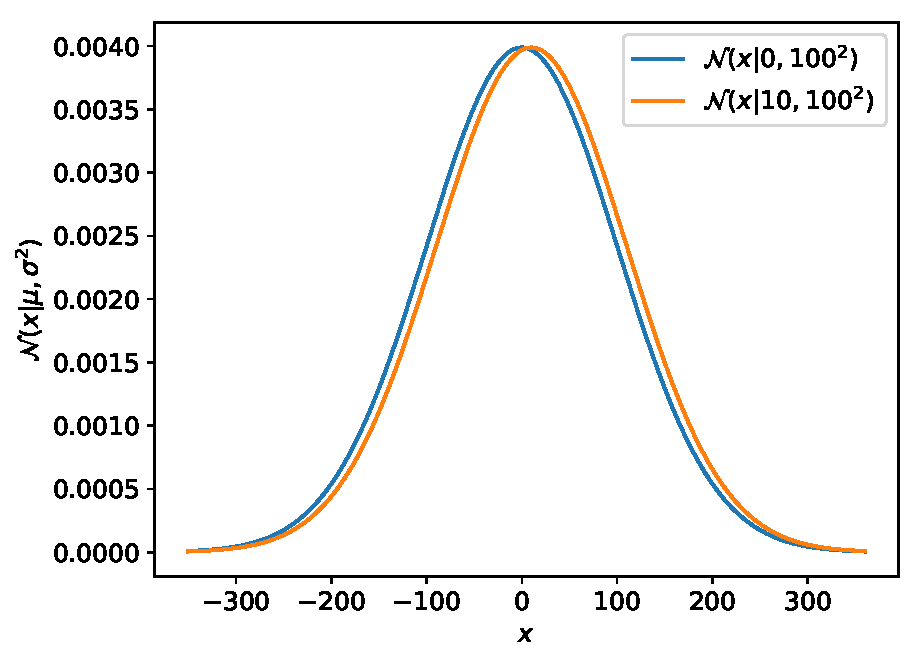
\includegraphics[height=5.2cm]{graphics/gaussian-pdfs/S1.pdf}
        \caption{}
        \label{fig: Theory: gaussian-pdfs/S1}
    \end{subfigure}
    \hfill
    \begin{subfigure}[b]{0.48\textwidth}
        \centering
        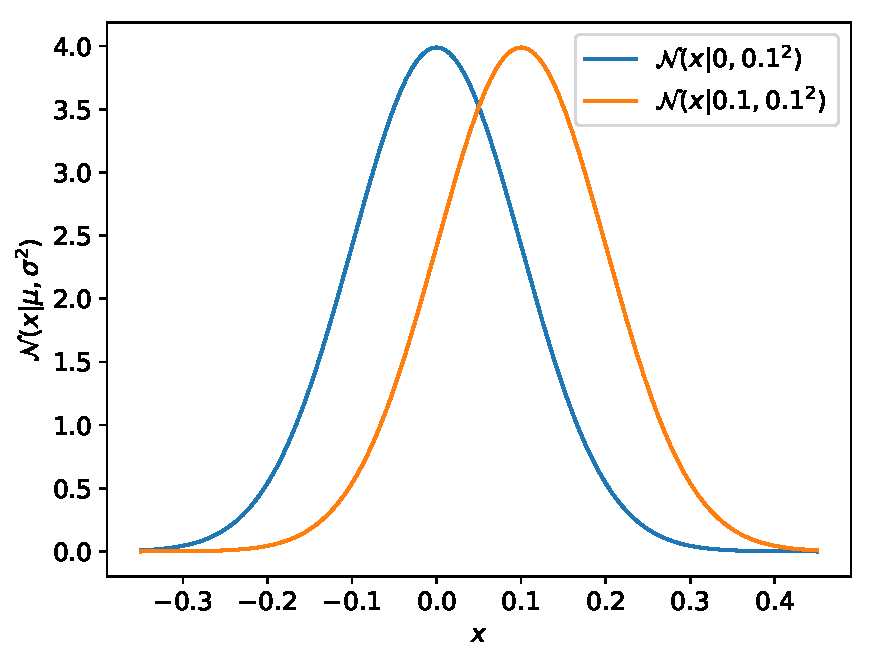
\includegraphics[height=5.2cm]{graphics/gaussian-pdfs/S2.pdf}
        \caption{}
        \label{fig: Theory: gaussian-pdfs/S2}
    \end{subfigure}
    \caption{
        Two pairs of univariate Gaussians, $P_1$ in \subref{fig: Theory: gaussian-pdfs/S1} and $P_2$ in \subref{fig: Theory: gaussian-pdfs/S2}. The $P_1$ pair is obviously very similar while the $P_2$ pair are somewhat dissimilar. A suitable measure of the dissimilarity of two probability distributions is expected to reflect this.
    }
    \label{fig: Theory: gaussian-pdfs}
\end{figure}

In the \gls{VO} setting, a search distribution is maintained over the network weights and it is updated iteratively using gradient descent. Evaluating the closeness of successive search distributions by computing the Euclidean distance between their parameter vectors can be shown to be give counter intuitive results. Take for instance the two pairs of univariate Gaussians shown in \autoref{fig: Theory: gaussian-pdfs},
\begin{align*}
    P_1 &= \cbra{\mathcal{N}(0,100^2), \mathcal{N}(10,100^2)}\\
    \shortintertext{and}
    P_2 &= \cbra{\mathcal{N}(0,0.1^2), \mathcal{N}(0.1,0.1^2)} \ .
\end{align*}
%$$P_1 = \cbra{\mathcal{N}(0,100^2), \mathcal{N}(10,100^2)}$$
%and
%$$P_2 = \cbra{\mathcal{N}(0,0.1^2), \mathcal{N}(0.1,0.1^2)}.$$
Due to their large variance, the first two distributions are almost identical while the other pair of distributions share limited support. As a consequence of their parameterizations however, the Euclidean distance, $D_2$, between the first pair is
$$D_\text{2}\pa{\mathcal{N}(0,100^2), \mathcal{N}(10,100^2)} = \sqrt{\pa{0-10}^2+\pa{100^2-100^2}^2}= 10$$
whereas the distance between the second pair is
$$D_\text{2}\pa{\mathcal{N}(0,0.1^2), \mathcal{N}(0.1,0.1^2)} = \sqrt{\pa{0-0.1}^2+\pa{0.1^2-0.1^2}^2}= 0.1,$$
a factor of 1000 lower. 

That Euclidean distance is an unsuited measure of closeness between probability distributions can be theoretically attributed to distributions not residing in a Euclidean space but rather on a Riemannian manifold (or statistical manifold) \cite{Suzuki2014}. Although this thesis will not delve further into the details of these manifolds, measuring distance within them must be done with respect to a form of distance metric. This is akin to relating a line segment $ds$ in Euclidean space to changes $dx$ and $dy$ in the $x$ and $y$ directions by the relation $ds=\sqrt{dx^2+dy^2}$ only here, $ds$ is a line segment on the statistical manifold and the directions represent parameters of a family of probability distributions, e.g. $\mu$ and $\sigma$ of the univariate Gaussian \cite{Suzuki2014}.


\subsection{The Kullback-Leibler divergence}\label{sec: Natural Gradient - KL divergence}
A better and more natural measure of distance between two probability distributions is the \glsfirst{KL} divergence. It is defined as \cite{Bishop2006}
\begin{align}
    D_\text{KL}(p||q)
    &= -\int p(\x)\log q(\x)\,\text{d}\x - \pa{-\int p(\x)\log p(\x)\,\text{d}\x} \nonumber\\
    &= -\int p(\x)\log\pa{\frac{q(\x)}{p(\x)}}\,\text{d}\x \ .\label{eq: Theory: Definition of KL divergence}
\end{align}
The \gls{KL} divergence satisfies $D_\text{KL}(p||q)\geq0$ with equality only when $p(\x)=q(\x)$ and it is asymmetrical such that $D_\text{KL}(p||q)\ne D_\text{KL}(q||p)$. As such is it strictly speaking not a measure of distance but should rather be interpreted as a measure of information loss by using $q$ rather than $p$ or, inversely, a measure of required additional information by using $q$ rather than $p$, to encode some amount of information. For example, in variational Bayesian methods, the \gls{KL} divergence is often used as the measure of dissimilarity between a distribution $q(\z)$ that approximates a posterior distribution $p(\z|\x)$ where $\x$ and $\z$ are respectively observed and unobserved (latent) variables. In fact, $q(\z)$ approximates Bayes' theorem
\begin{equation}
    p(\z|\x) = \frac{p(\x|\z)p(\z)}{p(\x)}
\end{equation}
in which the marginalization over $\z$ to compute $p(\x)$ is often intractable. The approximation is computed by minimizing the \gls{KL} divergence of the approximate posterior between the true posterior, $D_\text{KL}(q||p)$. The \gls{KL} divergence can then be seen as the average minimal additional amount of information required to specify the value of $\z$ as a result of using $q(\z)$ instead of $p(\z|\x)$\footnote{The information content is measured in bits if the base 2 logarithm is used and in nats if the natural logarithm is used. The relation between the two is $\SI{1}{nat}=\frac{1}{\ln 2}\si{bit} \approx \SI{1.44}{bit}$.} \cite{Bishop2006}.

A symmetrized version of the \gls{KL} divergence which satisfies $D_\text{KL}(p,q)=D_\text{KL}(q,p)$ can be defined as
\begin{align}
    D_\text{KL}(p,q)
    &= D_\text{KL}(p||q) + D_\text{KL}(q||p) \nonumber\\
    &= -\int p(\x)\log\pa{\frac{q(\x)}{p(\x)}}\,\text{d}\x - \int q(\x)\log\pa{\frac{p(\x)}{q(\x)}}\,\text{d}\x \nonumber\\
    &= \int p(\x)\log\pa{\frac{p(\x)}{q(\x)}}\,\text{d}\x - \int q(\x)\log\pa{\frac{p(\x)}{q(\x)}}\,\text{d}\x \nonumber\\
    &= \int \pa{p(\x)-q(\x)}\log\pa{\frac{p(\x)}{q(\x)}}\,\text{d}\x \ .\label{eq: Theory: Definition of symmetrized KL divergence}
\end{align}

The \gls{KL} divergence and the symmetrized \gls{KL} divergence between two univariate Gaussians, $\mathcal{N}(\mu_1,\sigma_1^2)$ and $\mathcal{N}(\mu_2,\sigma_2^2)$, are\footnote{For derivations, see \autoref{app: Regular and symmetrized Kullback-Leibler divergence for univariate Gaussian}}
\begin{align}
    D_\text{KL}\pa{\mathcal{N}(\mu_1,\sigma_1^2) || \mathcal{N}(\mu_2,\sigma_2^2)} &= \log\pfrac{\sigma_2}{\sigma_1} + \frac{\sigma_1^2+(\mu_1+\mu_2)^2}{2\sigma_2^2} - \frac{1}{2}\\
    D_\text{KL}\pa{\mathcal{N}(\mu_1,\sigma_1^2), \mathcal{N}(\mu_2,\sigma_2^2)} &= \pa{(\mu_1-\mu_2)^2 + (\sigma_1^2 + \sigma_2^2)}\pa{\frac{1}{2\sigma_1^2} + \frac{1}{2\sigma_2^2}} - 2 \ .
\end{align}
For the pairs, $P_1$ and $P_2$ considered above, the \gls{KL} divergence and symmetrized \gls{KL} divergence become
\begin{align}
    D_\text{KL}\pa{\mathcal{N}(0,100^2)||\mathcal{N}(10,100^2)} &= 0.005\nonumber\\
    D_\text{KL}\pa{\mathcal{N}(0,0.1^2)||\mathcal{N}(0.1,0.1^2)} &= 0.5\nonumber
\end{align}
and
\begin{align}
    D_\text{KL}\pa{\mathcal{N}(0,100^2), \mathcal{N}(10,100^2)} &= 0.01\nonumber\\
    D_\text{KL}\pa{\mathcal{N}(0,0.1^2), \mathcal{N}(0.1,0.1^2)} &= 1\nonumber \ ,
\end{align}
respectively. The ordering of the distributions in the regular \gls{KL} divergence is unimportant in this specific case since the asymmetry is in the variances and the variances are equal here. In both cases, this measure of dissimilarity is a factor of $100$ lower for the $P_1$ pair compared to the $P_2$ pair. Evidently, both the regular and symmetrized \gls{KL} divergence much better represent similarity between distributions than the Euclidean measure which, contrary to intuition, considered the $P_1$ pair to be much further apart than $P_2$.


\subsection{The Fisher information matrix}\label{sec: Natural Gradient - Fischer information matrix}
For the purposes of the following section, this section will consider how to compute an approximation to the \gls{KL} divergence.
For two distributions, $p(\x|\thetab)$ and $p(\x|\thetab+\Delta\thetab)$, that differ by some small vector $\Delta\thetab$ in their parameter vectors, a second order Taylor approximation to their symmetric \gls{KL} divergence can be computed as follows\footnote{This is derivation is intended to sketch the proof but is not a completely rigorous proof in itself.}. Let
$$\Delta p(\x|\thetab)=p(\x|\thetab+\Delta\thetab)-p(\x|\thetab)$$
and rewrite the symmetric \gls{KL} divergence as follows
\begin{align}
    D_\text{KL}(p(\x|\thetab+\Delta\thetab),p(\x|\thetab))
    &= \int \pa{p(\x|\thetab+\Delta\thetab)-p(\x|\thetab)}\log\pa{\frac{p(\x|\thetab+\Delta\thetab)}{p(\x|\thetab)}}\,\text{d}\x\nonumber\\
    &= \int \Delta p(\x|\thetab)\log\pa{1+\frac{\Delta p(\x|\thetab)}{p(\x|\thetab)}}\,\text{d}\x\nonumber\\
    &= \int p(\x|\thetab)\frac{\Delta p(\x|\thetab)}{p(\x|\thetab)}\log\pa{1+\frac{\Delta p(\x|\thetab)}{p(\x|\thetab)}}\,\text{d}\x \ .
\end{align}
Now, the Taylor expansion of the logarithm is
\begin{equation}
    \log (1+x) = \log(1) + x + \mathcal{O}(x^2)
    %\log (1+x) = \log(1) + x + \frac{1}{2}x^2 + \frac{1}{3}x^3 + \dots,
\end{equation}
which implies that
\begin{equation}
    \log\pa{1+\frac{\Delta p(\x|\thetab)}{p(\x|\thetab)}} \approx \frac{\Delta p(\x|\thetab)}{p(\x|\thetab)} \ .
\end{equation}
Applying this to the symmetric \gls{KL} divergence above yields
\begin{equation}
    D_\text{KL}p(\x|\thetab)(p(\x|\thetab+\Delta\thetab),p(\x|\thetab)) \approx \int p(\x|\thetab) \frac{\Delta p(\x|\thetab)}{p(\x|\thetab)}\frac{\Delta p(\x|\thetab)}{p(\x|\thetab)}\,\text{d}\x \ .
\end{equation}
Given that the parameter change $\Delta\thetab$ is small enough, $\nabla_\thetab p(\x|\thetab)\transpose\Delta\thetab$ will be a finite difference approximation to $\Delta p(\x|\thetab)$, i.e.
\begin{equation}
    \Delta p(\x|\thetab) \approx \nabla_\thetab p(\x|\thetab)\transpose\Delta\thetab \ .
\end{equation}
Substituting this approximation and using the log-derivative trick \eqref{eq: Theory: Log-derivative trick for pdf}, the symmetric \gls{KL} divergence becomes
\begin{align}
    D_\text{KL}(p(\x|\thetab+\Delta\thetab),p(\x|\thetab))
    % &\approx \int p(\x|\thetab)\bra{
    % \Delta\thetab\transpose\frac{\nabla_\thetab p(\x|\thetab)}{p(\x|\thetab)}}\bra{
    % \frac{\nabla_\thetab p(\x|\thetab)\transpose}{p(\x|\thetab)}\Delta\thetab}\,\text{d}\x\nonumber\\
    &\approx \int p(\x|\thetab)
    \Delta\thetab\transpose\frac{\nabla_\thetab p(\x|\thetab)}{p(\x|\thetab)}
    \frac{\nabla_\thetab p(\x|\thetab)\transpose}{p(\x|\thetab)}\Delta\thetab\,\text{d}\x\nonumber\\
    &= \int p(\x|\thetab)
    \Delta\thetab\transpose\nabla_\thetab\log p(\x|\thetab)
    \nabla_\thetab\log p(\x|\thetab)\transpose\Delta\thetab\,\text{d}\x\nonumber\\
    &= \Delta\thetab\transpose\int p(\x|\thetab)
    \nabla_\thetab\log p(\x|\thetab)
    \nabla_\thetab\log p(\x|\thetab)\transpose\,\text{d}\x\; \Delta\thetab \ .
\end{align}
Note that the integral is an expectation with respect to $p(\x|\thetab)$ of the outer product of the gradient of the log-\gls{PDF} of the search distribution. This can be seen to be the \glsfirst{FIM} which is defined as \cite{Bishop2006}
\begin{equation}\label{eq: Theory: Fischer information matrix definition}
    \F_\thetab
    = \text{E}\bra{\nabla_\thetab\log p(\x|\thetab)\nabla_\thetab\log p(\x|\thetab)\transpose}_{p(\x|\thetab)} \ .
\end{equation}
Using the \gls{FIM}, the approximate symmetric \gls{KL} divergence can thus be written as
\begin{equation}\label{eq: Theory: Second order approximation to the symmetric KL divergence}
    D_\text{KL}(p(\x|\thetab+\Delta\thetab),p(\x|\thetab)) \approx \Delta\thetab\transpose\F_\thetab\Delta\thetab \ .
\end{equation}
Under certain regularity conditions which will not be discussed here, the \gls{FIM} can also be written as \cite{Ly2017}
\begin{equation}\label{eq: Theory: Fischer information matrix definition (for computation)}
    \F_\thetab = - \text{E}\bra{\H_\thetab\log p(\x|\thetab)} = \text{Cov}\bra{\nabla_\thetab\log p(\x|\thetab)}
\end{equation}
which is useful for computation.


\subsection{Steepest descent w.r.t. a distance metric}\label{sec: Natural Gradient: Steepest descent w.r.t. a distance metric}
\autoref{sec: Natural Gradient} set out to understand what makes the regular gradient suboptimal for gradient descent in \glsfirst{VO}. Now that it is clear why Euclidean distance is unsuited and the \gls{KL} divergence has been introduced and substantiated as a more fitting measure of similarity between distributions, this section will derive the natural gradient by imposing a constraint on the dissimilarity between the updated and previous search distributions. To demonstrate the relation between the regular and natural gradients, the regular gradient will be derived first in an unconstrained manner and by imposing a Euclidean dissimilarity constraint.

At each iteration of \gls{VO}, a direction $\Delta\thetab$ is sought that minimizes the variational upper bound. With no constraints on the update this can be expressed as the following unconstrained minimization problem.
\begin{equation}\label{eq: Theory: Unconstrained VO optimization problem at each iteration}
    \min_{\Delta\thetab} U(\thetab+\Delta\thetab) \approx U(\thetab) + \nabla_\thetab U(\thetab)\transpose\Delta\thetab + \frac{1}{2}\Delta\thetab\transpose\H_\thetab U(\thetab)\transpose\Delta\thetab \ ,
\end{equation}
which uses a second order Taylor expansion of the variational upper bound around the current parameter $\thetab$. The solution to this problem is found by taking the gradient w.r.t. $\Delta\thetab$ of the objective,
\begin{equation}
    \nabla_{\Delta\thetab}\bra{U(\thetab) + \nabla_\thetab U(\thetab)\transpose\Delta\thetab + \frac{1}{2}\Delta\thetab\transpose\nabla_\thetab U(\thetab)\transpose\Delta\thetab} = \nabla_\thetab U(\thetab) + \H_\thetab U(\thetab)\Delta\thetab,
\end{equation}
setting it to zero and solving for $\Delta\thetab$. This yields
\begin{equation*}
    \Delta\thetab = -\H_\thetab U(\thetab)^{-1}\nabla_\thetab U(\thetab)
\end{equation*}
which is the well-known Newton search direction. In cases where Hessian information is not available or computationally intractable, it can be ignored and a fixed learning rate used on the gradient instead giving the search direction
\begin{equation}
    \Delta\thetab = -\eta\nabla_\thetab U(\thetab) \ .
\end{equation}

Alternatively, a constraint can be imposed on the optimization problem in \eqref{eq: Theory: Unconstrained VO optimization problem at each iteration}. For instance, constraining the Euclidean distance $D_2(\cdot)$ between parameters $\thetab$ and $\thetab+\Delta\thetab$ to be some small constant $\kappa^2$, the problem becomes,
\begin{equation}\label{eq: Theory: Constrained VO optimization problem at each iteration (Euclidean dissimilarity)}
    \begin{aligned}
        \min_{\Delta\thetab} &\; U(\thetab+\Delta\thetab) \approx U(\thetab) + \nabla_\thetab U(\thetab)\transpose\Delta\thetab\\
        \text{subject to} &\; D_2(\thetab+\Delta\thetab, \thetab) = \sqrt{\Delta\thetab\transpose\Delta\thetab} = \kappa^2 \ ,
    \end{aligned}
\end{equation}
where only a first order Taylor approximation has been used since second order dependencies are introduced in the constraint. Such a problem is solved using the methods of constrained optimization \cite{Nocedal2006}. Writing the Euclidean constraint as $\Delta\thetab\transpose\Delta\thetab = \kappa$, the Lagrangian for the problem becomes
\begin{equation}
    \mathcal{L}(\thetab,\lambda) = U(\thetab) + \nabla_\thetab U(\thetab)\transpose\Delta\thetab - \lambda\pa{\Delta\thetab\transpose\Delta\thetab - \kappa}
\end{equation}
which is minimized w.r.t. $\Delta\thetab$
\begin{equation*}
    0 = \nabla_{\Delta\thetab}\mathcal{L}(\thetab,\lambda) = \nabla_\thetab U(\thetab) - \lambda\Delta\thetab
\end{equation*}
yielding
\begin{equation}
    \Delta\thetab = \lambda^{-1}\nabla_\thetab U(\thetab) \ .
\end{equation}
The Lagrange multiplier $\lambda$ can be found by first forming the dual of the Lagrangian by insertion of the result into the primal Lagrangian and then minimizing the dual w.r.t. the multiplier. The dual Lagrangian becomes
\begin{align}
    \mathcal{L}_d(\lambda)
    &= U(\thetab) + \lambda^{-1}\nabla_\thetab U(\thetab)\transpose\nabla_\thetab U(\thetab) - \lambda\kappa\nonumber\\
    &= U(\thetab) + \lambda^{-1}\nabla^2_\thetab U(\thetab) - \lambda\kappa\nonumber
\end{align}
where $\nabla^2$ denotes the vector Laplacian. Differentiate the Lagrangian w.r.t. $\lambda$ and set it to zero,
\begin{equation*}
    0 = \frac{d}{d\lambda}\mathcal{L}_d(\lambda) = -\lambda^{-2}\nabla^2_\thetab U(\thetab) - \kappa \ .
\end{equation*}
Finally solve for $\lambda$ to obtain
\begin{equation}
    \lambda = - \sqrt{\frac{\nabla^2_\thetab U(\thetab)}{\kappa}} \ .
\end{equation}
The search direction then becomes
\begin{equation}
    \Delta\thetab = - \sqrt{\frac{\kappa}{\nabla^2_\thetab U(\thetab)}}\nabla_\thetab U(\thetab) = -\eta\nabla_\thetab U(\thetab)
\end{equation}
where $\eta=\sqrt{\frac{\kappa}{\nabla^2_\thetab U(\thetab)}}$ is some potentially undesirable learning rate that can be replaced by a constant without changing the search direction. Note that this constrained approach has resulted in the emergence of the negative regular gradient as the optimal descent direction for minimization while constraining step sizes to be constant in the sense of Euclidean distance.

Rather than using the Euclidean distance between distribution parameters as the measure of dissimilarity between the distributions, now the approximate symmetrized \gls{KL} divergence defined in \eqref{eq: Theory: Definition of symmetrized KL divergence} is used to impose the dissimilarity constraint in \eqref{eq: Theory: Constrained VO optimization problem at each iteration (Euclidean dissimilarity)}. The minimization problem is then given by,
\begin{equation}\label{eq: Theory: Constrained VO optimization problem at each iteration (KL divergence dissimilarity)}
    \begin{aligned}
        \min_{\Delta\thetab} &\; U(\thetab+\Delta\thetab) \approx U(\thetab) + \nabla_\thetab U(\thetab)\transpose\Delta\thetab\\
        \text{subject to} &\; D_\text{KL}\pa{p(\x|\thetab+\Delta\thetab), p(\x|\thetab)} \approx \frac{1}{2}\Delta\thetab\transpose\F_\thetab\Delta\thetab = \kappa \ ,
    \end{aligned}
\end{equation}
where $p(\x|\thetab)$ is the used search distribution.
As discussed earlier, the dissimilarity constraint now takes the form of a distance w.r.t. a distance metric, here, the \gls{FIM}. In fact, the \gls{FIM} measures closeness of the shape of two distributions and is proportional to the amount of information that the distribution function contains about the parameter. As such, it provides a distance metric on the statistical manifold \cite{Suzuki2014}.
Again, to obtain the optimal search direction, the Lagrangian is formed,
\begin{equation}
    \mathcal{L}(\thetab,\lambda) = U(\thetab) + \nabla_\thetab U(\thetab)\transpose\Delta\thetab - \lambda\pa{\frac{1}{2}\Delta\thetab\transpose\F_\thetab\Delta\thetab - \kappa} \ ,
\end{equation}
differentiated w.r.t. $\Delta\thetab$ and set equal to zero,
\begin{equation}
    0 = \nabla_\thetab\mathcal{L}(\thetab,\lambda) = \nabla_{\Delta\thetab} U(\thetab) - \lambda\F_\thetab\Delta\thetab \ ,
\end{equation}
and finally solved for $\Delta\thetab$ to yield
\begin{equation}
    \Delta\thetab = \lambda^{-1}\F_\thetab^{-1}\nabla_\thetab U(\thetab) \ .
\end{equation}
Again, the Lagrange multiplier $\lambda$ can be found by minimizing the dual Lagrangian,
\begin{equation}
    \mathcal{L}_d(\lambda) = U(\thetab) + \lambda^{-1} \nabla_\thetab U(\thetab)\transpose\F_\thetab^{-1}\nabla_\thetab U(\thetab) - \lambda\kappa \ ,
\end{equation}
w.r.t the multiplier,
\begin{equation}
    0 = \frac{d}{d\lambda}\mathcal{L}_d(\lambda) = -\lambda^{-2} \nabla_\thetab U(\thetab)\transpose\F_\thetab^{-1}\nabla_\thetab U(\thetab) - \kappa \ ,
\end{equation}
and solving for $\lambda$,
\begin{equation}
    \lambda = -\sqrt{\frac{\nabla_\thetab U(\thetab)\transpose\F_\thetab^{-1}\nabla_\thetab U(\thetab)}{\kappa}} \ .
\end{equation}
The search direction is then
\begin{equation}
    \Delta\thetab = -\sqrt{\frac{\kappa}{\nabla_\thetab U(\thetab)\transpose\F_\thetab^{-1}\nabla_\thetab U(\thetab)}}\F_\thetab^{-1}\nabla_\thetab U(\thetab) = -\eta\F_\thetab^{-1}\nabla_\thetab U(\thetab)
\end{equation}
where $\eta=\sqrt{\frac{\kappa}{\nabla_\thetab U(\thetab)\transpose\F_\thetab^{-1}\nabla_\thetab U(\thetab)}}$ is an arbitrary learning rate as before. This search direction is the optimal direction of descent for minimization of the objective while satisfying the constraint that the updated distribution is dissimilar from the previous distribution only by a constant amount as measured by the symmetric \gls{KL} divergence. This search direction is precisely the natural gradient originally introduced in \cite{Amari1998}.

The natural gradient is thus computed by rescaling the regular gradient with the inverse \gls{FIM}. Since the \gls{FIM} is a positive semi-definite matrix it has $n(n+1)/2$ unique entries for a distribution with $n$ parameters. This can in some cases be intractable to store and compute. For example, for an \gls{NN} optimized with \gls{VO} using a $d$-dimensional multivariate Gaussian with full covariance matrix $n=(d+d(d+1)/2)=\mathcal{O}(d^2)$ and the number of elements in the \gls{FIM} is $\mathcal{O}(d^4)$. 
% , the number of parameters in the \gls{FIM} may be as high as
% $$(d+d(d+1)/2)(d+d(d+1)/2) = \frac{1}{4}(d^2 + 3d)^2$$
% which scales as $\mathcal{O}(d^4)$. 
However, in some interesting special cases, the \gls{FIM} has much fewer unique parameters. Below, such distributions are considered. 

In \cite{Wierstra2008}, an additional abstraction is made for a general class of rotationally symmetric distributions (which includes the Gaussian) by introduction of ``exponential local natural coordinates". This constitutes a reparameterization of the search distribution that results in the \gls{FIM} becoming the identity and the gradient thus automatically being the natural one. This has not been considered further here but could reduce computation when using the natural gradient with distributions with e.g. covariances.

\iffalse
\textbf{- Steepest Descent with Respect to a Metric N derived by minimizing objective while keeping distance to new parameters equal to constant}
- \url{http://www.ias.tu-darmstadt.de/uploads/Research/Thesis/thesiP_1.pdf} page 75 for solution of minimization of distance between probability distributions.

% http://people.missouristate.edu/songfengzheng/Teaching/MTH541/Lecture%20notes/Fisher_info.pdf
% https://en.wikipedia.org/wiki/Fisher_information

\cite{Peters2007}

\url{https://hips.seas.harvard.edu/blog/2013/01/25/the-natural-gradient/}

\url{http://kvfrans.com/what-is-the-natural-gradient-and-where-does-it-appear-in-trust-region-policy-optimization/}

Natural gradient introduced by \cite{Amari1998}

Wierstra Natural Evolution Strategies \cite{Wierstra2008}


\begin{align}
    D_\text{KL}(p_\thetab||p_{\thetab+\Delta\thetab})
    &= D_\text{KL}(\Delta\thetab)\\
    &\approx D_\text{KL}(0) + \Delta\thetab\transpose\nabla_\thetab D_\text{KL}(0) + \frac{1}{2}\Delta\thetab\transpose\nabla^2_\thetab D_\text{KL}(0)\Delta\thetab\\
    &= 0 + (0?) + Something Fischer matrix kinda\\ 
    &= D_\text{KL}(p_\thetab||p_{\thetab})\\
    &= NEED CALCULATIONS HERE\\
    &= \frac{1}{2}\Delta\thetab\transpose\bra{\int p_\thetab(\x)\nabla^2_\thetab\log p_\thetab(\x)\transpose\,\text{d}\x}\Delta\thetab\\
    &= \frac{1}{2}\Delta\thetab\transpose\bra{-\int p_\thetab(\x)\nabla_\thetab\log p_\thetab(\x)\nabla_\thetab\log p_\thetab(\x)\,\text{d}\x}\Delta\thetab\\
    &= \frac{1}{2}\Delta\thetab\transpose\F_\thetab\Delta\thetab
\end{align}
\fi


\subsection{Natural gradient for different search distributions}
This section derives the \gls{FIM} and the associated natural gradient for the univariate, isotropic and separable Gaussian search distributions.


\subsubsection{Univariate Gaussian}
The \gls{FIM} for a univariate Gaussian can be computed as follows. Since the univariate Gaussian has two parameters, the \gls{FIM} will be a $2\times2$ matrix. The derivatives of the Gaussian log-\gls{PDF} were computed in \eqref{eq: Theory: Variational optimization univariate gaussian search gradients} with which the gradient of the univariate Gaussian w.r.t. to its parameter vector $\thetab=\bmat{\mu & \sigma^2}^\text{T}$ can be constructed as
\begin{equation}
    \nabla_\thetab\log\mathcal{N}(x|\mu,\sigma^2) = \bmat{\frac{1}{\sigma^2}(x-\mu) \\ -\frac{1}{2\sigma^2}+\frac{1}{2\sigma^4(x-\mu)^2}} \ .
\end{equation}
Its Hessian is then
\begin{equation}
    \H_\thetab\log\mathcal{N}(x|\mu,\sigma^2) = \bmat{-\frac{1}{\sigma^2} & -\frac{1}{\sigma^4}(x-\mu) \\ -\frac{1}{\sigma^4}(x-\mu) & \frac{1}{2\sigma^4}-\frac{1}{\sigma^6}(x-\mu)^2} \ .
\end{equation}
With $\text{E}\bra{x-\mu}=0$ and $\text{E}\bra{(x-\mu)^2}=\sigma^2$ and using \eqref{eq: Theory: Fischer information matrix definition (for computation)}, the \gls{FIM} then becomes
\begin{equation}
    \F_\thetab = -\text{E}\bra{\H_\thetab\log\mathcal{N}(x|\mu,\sigma^2)} = \bmat{\frac{1}{\sigma^2} & 0 \\ 0 & \frac{1}{2\sigma^4}}
\end{equation}
and the inverse \gls{FIM} required for the natural gradient is easily obtained,
\begin{equation}
    \F_\thetab^{-1} = \bmat{\sigma^2 & 0 \\ 0 & 2\sigma^4} \ .
\end{equation}
The natural gradient version of the \gls{VO} gradient estimator in \eqref{eq: Theory: Variational optimization univariate gaussian gradient estimators} therefore becomes
\begin{equation}
    \begin{aligned}
        \sigma^2\pderiv{}{\mu}U(\mu,\sigma^2) &= \sigma\text{E}\bra{f(\mu + \sigma\epsilon)\epsilon} \approx \frac{\sigma}{N}\sum_{n=1}^N f(\mu+\sigma\epsilon_n)\epsilon_n\\
        2\sigma^4\pderiv{}{\sigma^2}U(\mu,\sigma^2) &= \sigma^2\text{E}\bra{f(\mu + \sigma\epsilon)\left(\epsilon^2-1\right)} \approx \frac{\sigma^2}{N}\sum_{n=1}^N f(\mu + \sigma\epsilon_n)\left(\epsilon_n^2-1\right)\\
    \end{aligned}\label{eq: Theory: Variational optimization univariate gaussian gradient estimators (natural gradient)}
\end{equation}
where $\epsilon\sim\mathcal{N}(0,1)$. These evidently posses the desired property that the gradient goes to zero as the variance goes to zero and the opposite.


\subsubsection{Isotropic Gaussian}
A $d$-dimensional isotropic Gaussian, $\mathcal{N}(\mub,\sigma^2\I)$, has $d+1$ parameters which implies that the \gls{FIM} will be a $(d+1)\times(d+1)$ matrix. The gradients of the log-\gls{PDF} of the isotropic Gaussian were derived in \eqref{eq: Theory: Variational optimization multivariate isotropic gaussian search gradients}. 
The gradient of the isotropic Gaussian w.r.t. to its parameter vector $\thetab=\bmat{\mub & \sigma^2}^\text{T}$ can then be constructed as
\begin{equation}
    \nabla_\thetab\log\mathcal{N}(\x|\mub,\sigma^2\I) = \bmat{\frac{1}{\sigma^2}(\x-\mub) \\ -\frac{d}{2\sigma^2} + \frac{1}{2\sigma^4}(\x-\mub)\transpose(\x-\mub)} \ .
\end{equation}
It follows that the Hessian is
\begin{equation}
    \H_\thetab\log\mathcal{N}(\x|\mub,\sigma^2\I) = \bmat{-\frac{1}{\sigma^2}\I & -\frac{1}{\sigma^4}(\x-\mub) \\ -\frac{1}{\sigma^4}(\x-\mub) & \frac{d}{2\sigma^4}-\frac{1}{\sigma^6}(\x-\mub)\transpose(\x-\mub)} \ .
\end{equation}
Again, use \eqref{eq: Theory: Fischer information matrix definition (for computation)} to compute the \gls{FIM} and exploit that $\text{E}\bra{\x-\mub}=\0$ and $\text{E}\bra{(\x-\mub)\transpose(\x-\mub)}=d\sigma^2$ to obtain\footnote{This follows from the following argument.
\begin{align}
    \text{E}\bra{(\x-\mub)\transpose(\x-\mub)} = \text{E}\bra{\x\transpose\x}-\text{E}\bra{\x\transpose\mub}-\text{E}\bra{\mub\transpose\x}+\text{E}\bra{\mub\transpose\mub}
    = \text{E}\bra{\x\transpose\x} - \mub\transpose\mub \ .\nonumber
\end{align}
Now, when $\x\sim\mathcal{N}(\mu,\sigma^2\I)$
\begin{align}
    \text{E}\bra{\x\transpose\x} &= \text{E}\bra{\sum_{i=1}^d x_i^2}
    = \sum_{i=1}^d \text{E}\bra{x_i^2}
    = \sum_{i=1}^d \text{Var}\bra{x_i}+\text{E}\bra{x_i}^2
    = \sum_{i=1}^d \sigma^2+\mu_i^2
    = d\sigma^2+\mub\transpose\mub\nonumber \ ,
\end{align}
such that
\begin{align}
    \text{E}\bra{(\x-\mub)\transpose(\x-\mub)} &= d\sigma^2\nonumber \ .
\end{align}
}
\begin{equation}
    \F_\thetab = \bmat{\frac{1}{\sigma^2}\I & 0 \\ 0 & \frac{1}{2\sigma^4}} \Longleftrightarrow \F_\thetab^{-1} = \bmat{\sigma^2\I & 0 \\ 0 & 2\sigma^4} \ .
\end{equation}
%The inverse \gls{FIM} required for the natural gradient is easily obtained,
% \begin{equation}
%     \F_\thetab^{-1} = \bmat{\sigma^2\I & 0 \\ 0 & 2\sigma^4}.
% \end{equation}
This is simply the univariate result in each dimension of the mean while the result for the scalar variance parameter remains unchanged.
The natural gradient version of the \gls{VO} gradient estimator in \eqref{eq: Theory: Variational optimization multivariate isotropic gaussian gradient estimators} therefore becomes
\begin{equation}
    \begin{aligned}
        \sigma^2\nabla_\mub U(\mub,\sigma^2) &= \sigma\text{E}\bra{f(\mub + \sigma\epsilonb)\epsilonb} \approx \frac{\sigma}{N}\sum_{n=1}^N f(\mub+\sigma\epsilonb_n)\epsilonb_n\\
        2\sigma^4\nabla_{\sigmab^2} U(\mub,\sigma^2) &= \sigma^2\text{E}\bra{f(\mub + \sigma\epsilonb)\left(\epsilonb\transpose\epsilonb-d\right)} \approx \frac{\sigma^2}{N}\sum_{n=1}^N f(\mub + \sigma\epsilonb_n)\left(\epsilonb_n^2-d\right)\\
    \end{aligned}\label{eq: Theory: Variational optimization multivariate isotropic gaussian gradient estimators (natural gradient)}
\end{equation}
where $\epsilon\sim\mathcal{N}(\0,\I)$. The transformation applied to the \gls{VO} gradient using the isotropic Gaussian is clearly identical to the one applied to the gradient using a univariate Gaussian; in both cases the mean and variance gradients are multiplied by the scalars $\sigma^2$  and $2\sigma^4$, respectively.



\subsubsection{Separable Gaussian}
A $d$-dimensional separable Gaussian, $\mathcal{N}\pa{\x|\mub, (\sigmab^2\e\transpose)\odot\I}$, has $2d$ parameters which implies that the \gls{FIM} will be a $2d\times2d$ matrix. The gradients of the log-\gls{PDF} of the separable Gaussian were derived in \eqref{eq: Theory: Variational optimization multivariate isotropic gaussian search gradients (mub)} and \eqref{eq: Theory: Variational optimization multivariate isotropic gaussian search gradients (sigmab^2)}.
The gradient of the separable Gaussian w.r.t. its parameter vector $\thetab=\bmat{\mub & \sigmab^2}^\text{T}$ can then be constructed as
\begin{equation}
    \nabla_\thetab\log\mathcal{N}\pa{\x|\mub, (\sigmab^2\e\transpose)\odot\I} = \bmat{\sigmab^{-2} \odot (\x-\mub) \\  -\frac{1}{2}\sigmab^{-2} + \frac{1}{2} \sigmab^{-4}\odot(\x-\mub)^2} \ .
\end{equation}
It follows that the Hessian is
\begin{equation}
    \H_\thetab\log\mathcal{N}\pa{\x|\mub, (\sigmab^2\e\transpose)\odot\I} = \bmat{\sigmab^{-2} \odot\I & -\sigmab^{-4}\odot(\x-\mub) \\ -\sigmab^{-4}\odot(\x-\mub) & \frac{1}{2}\sigmab^{-4}-\sigmab^{-6}\odot(\x-\mub)^2} \ .
\end{equation}
Again, use \eqref{eq: Theory: Fischer information matrix definition (for computation)} to compute the \gls{FIM} and exploit that $\text{E}\bra{\x-\mub}=\0$ and $\text{E}\bra{(\x-\mub)^2}=\sigmab^2$ to obtain
\begin{equation}
    \F_\thetab = \bmat{\sigmab^{-2}\odot\I & 0 \\ 0 & \frac{1}{2}\sigmab^{-4}\odot\I} \Longleftrightarrow \F_\thetab^{-1} = \bmat{\sigmab^{2}\odot\I & 0 \\ 0 & 2\sigmab^{4}\odot\I} \ .
\end{equation}
% and, due to $F_{\thetab}$ being diagonal,
% \begin{equation}
%     \F_\thetab^{-1} = \bmat{\sigmab^{2}\odot\I & 0 \\ 0 & 2\sigmab^{4}\odot\I}.
% \end{equation}
Once again, this is the univariate result in each dimension of the parameter vector of the separable Gaussian. The natural gradient version of the \gls{VO} gradient estimator in \eqref{eq: Theory: Variational optimization separable gaussian gradient estimators} therefore becomes
\begin{equation}
    \begin{aligned}
        \sigmab^{2}\odot\nabla_\mub U(\mub,\sigma^2) &= \sigmab\odot\text{E}\bra{f(\mub + \sigmab\odot\epsilonb)\epsilonb}\\
        &\approx \sigmab\odot\frac{1}{N}\sum_{n=1}^N f(\mub+\sigmab\odot\epsilonb_n)\epsilonb_n\\
        2\sigmab^{4}\odot\nabla_\sigma^2 U(\mub,\sigma^2) &= \sigmab^{2}\odot\text{E}\bra{f(\mub + \sigmab\odot\epsilonb)\pa{\epsilonb^2 - 1}}\\
        &\approx \sigmab^{2}\odot\frac{1}{N}\sum_{n=1}^N f(\mub + \sigmab\odot\epsilonb_n)\pa{\epsilonb_n^2 - 1}\\
    \end{aligned}\label{eq: Theory: Variational optimization separable gaussian gradient estimators (natural gradient)}
\end{equation}
where $\epsilon\sim\mathcal{N}(\0,\I)$. The transformation applied here is again similar to the one applied to the gradient using a univariate Gaussian.


%If any two parameters, $\theta_i$ and $\theta_j$ are independent, the \gls{FIM} will contain a zero at the $(i,j)$'th entry, i.e. $\F_{ij}=0$. Clearly then if all parameters are independent, the \gls{FIM} will be diagonal.

% \subsection{Natural gradient for Cauchy search distributions}
% \begin{equation}
%     f(x;x_{0},\gamma )={\frac  {1}{\pi \gamma \left[1+\left({\frac{x-x_{0}}{\gamma}}\right)^{2}\right]}}=\frac{1}{\pi \gamma }\left[\frac{\gamma ^{2}}{ (x-x_{0})^{2}+\gamma ^{2}}\right],
% \end{equation}
% Since the Cauchy distribution has undefined moments, the Fischer information matrix is undefined in this case. However 
% \url{https://projecteuclid.org/download/pdfview_1/euclid.bjps/1291387776}

% Relation to CMA-ES \cite{Hansen2016} and TR-CMA-ES \cite{Abdolmaleki2017} as related methods that are more heuristic and less principled.

% \todo[inline]{Write section on natural gradient for Cauchy distribution (only if included earlier and useful)}



\subsection{Comparison of regular and natural gradients}\label{sec: Natural Gradient: Comparison of regular and natural gradients}
\begin{figure}[tbp!]
    \begin{subfigure}[b]{0.49\textwidth}
        \centering
        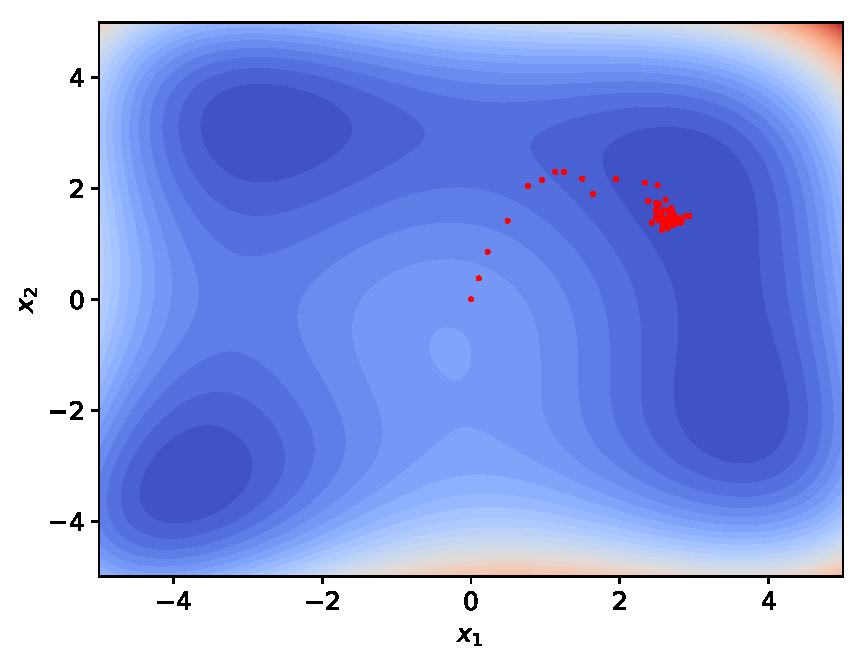
\includegraphics[height=5.8cm]{graphics/var-opt-conv/ES-himmelblau-convergence.pdf}
        \caption{}
        \label{fig: Theory: var-opt-conv-ES-himmelblau-convergence}
    \end{subfigure}
    \hfill
    \begin{subfigure}[b]{0.49\textwidth}
        \centering
        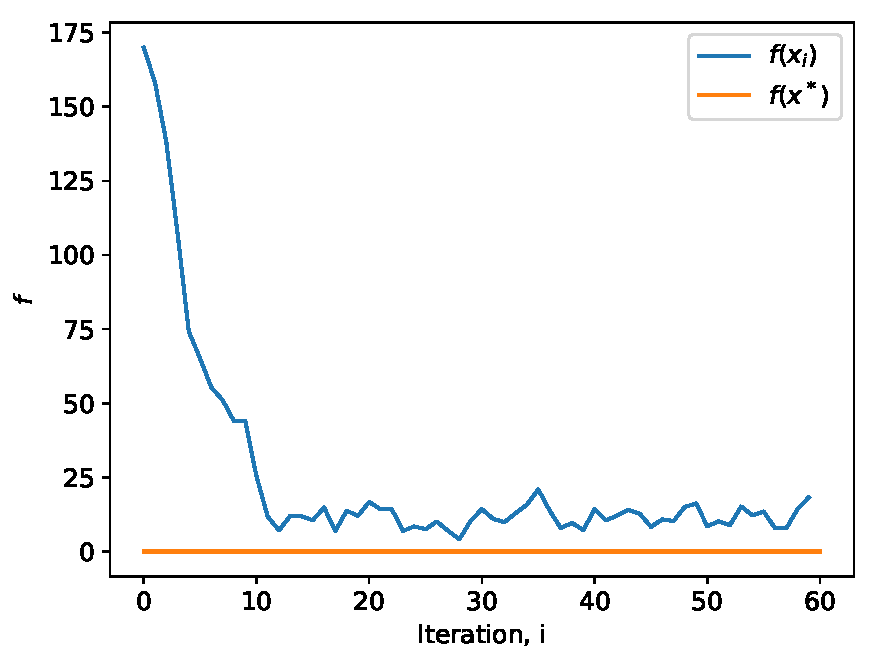
\includegraphics[height=5.8cm]{graphics/var-opt-conv/ES-himmelblau-f.pdf}
        \caption{}
        \label{fig: Theory: var-opt-conv-ES-himmelblau-f}
    \end{subfigure}
    \caption{\subref{fig: Theory: var-opt-conv-ES-himmelblau-convergence} Convergence on Himmelblau's function of the algorithm used by \cite{Salimans2017} with no adaptation of the variance. As in earlier contours, red denotes high values, blue denotes low values and the darker the colour, the higher the absolute value. The actual values are omitted for simplicity. \subref{fig: Theory: var-opt-conv-ES-himmelblau-f} Objective function value at each iteration of the algorithm. The algorithm finds a minimum but struggles to converge due to the fixed search distribution variance.}
    \label{fig: Theory: var-opt-conv-ES-himmelblau}
\end{figure}
In Figures \ref{fig: Theory: var-opt-conv-ES-himmelblau}, \ref{fig: Theory: var-opt-conv-VO-R-himmelblau} and \ref{fig: Theory: var-opt-conv-VO-N-himmelblau}, different versions of the variational optimization algorithm listed in \autoref{alg: Canonical variational optimization} are compared on Himmelblau's function. Himmelblau's function is two-dimensional objective function with four global minima and a local maximum. In these figures as before, red denotes high values, blue denotes low values and the darker the colour, the higher the absolute value. The actual values are omitted for simplicity.


In \autoref{fig: Theory: var-opt-conv-ES-himmelblau}, the convergence of the algorithm used in \cite{Salimans2017} and derived in \eqref{eq: Theory: Taylor: Multivariate gradient estimate from standard Gaussian} is shown. This algorithm estimates the regular gradient and does not adapt the value of the Gaussian search distribution variance. In \subref{fig: Theory: var-opt-conv-ES-himmelblau-convergence}, the iteration sequence is plotted on the contours of the objective function while in \subref{fig: Theory: var-opt-conv-ES-himmelblau-f}, the corresponding objective function value at each iteration is shown along with the global minimum value. Evidently, this algorithm quickly homes in on one of the global minima and stays in its vicinity for succeeding iterations. The objective function value reaches low values, but the fixed size of the variance results in it fluctuating above the global minimum never converging on it.

\autoref{fig: Theory: var-opt-conv-VO-R-himmelblau} presents the convergence of the \gls{VO} algorithm using an isotropic Gaussian search distribution. The used estimators for the regular gradients of the mean and variance are those in \eqref{eq: Theory: Variational optimization multivariate isotropic gaussian gradient estimators}. Similarly to the fixed variance version, this algorithm also quickly homes in on a minimum. However, the optimization of the variance results in increasingly smaller variances for each iteration. As previously discussed and and as expected, this increasingly smaller variance can be seen to give rise to increasingly larger gradient estimates. In the limit of zero variance (close to the minimum), the gradients explode and the function value starts increasing.

Finally, \autoref{fig: Theory: var-opt-conv-VO-N-himmelblau} presents the convergence of the same \gls{VO} algorithm using instead the natural gradient. The \gls{VO} natural gradient estimators for the univariate Gaussian used here are those in \eqref{eq: Theory: Variational optimization univariate gaussian gradient estimators (natural gradient)}. The minimum is found as before but this time the optimization of the variance drives the gradients to zero at the minimum resulting in much better convergence. Although the direction of the natural gradient is not different from the regular gradient for this specific type of search distribution, the gradient is much more well-behaved as $\sigma$ decreases.

These examples clearly demonstrate the differences between the methods and highlights \gls{VO} with natural gradients as the best choice for this problem. Replacing the regular gradient with the natural gradient results in better numerics for the estimators and convergence to the minimum. It should however be noted that Himmelblau's function is a low-dimensional objective function and the number of perturbations is much larger than the dimensionality for this example. This is fundamentally different from the optimization of \glspl{NN} by search in the extremely high-dimensional parameter space.

It can be noted that Gaussian \gls{VO} with fixed variance as in \autoref{fig: Theory: var-opt-conv-ES-himmelblau} in fact optimizes for the expected fitness of the entire population of perturbations rather than the fitness of the search distribution center \cite{Lehman2017}. As such, the fitness of the center of the search distribution (the unperturbed individual) may not be optimal at all although it often is close to the optimum, at least in terms of search space distance. This also results in solutions that exhibit robustness to small perturbations to the parameters \cite{Lehman2017}.
\begin{figure}[tbp!]
    \begin{subfigure}[b]{0.49\textwidth}
        \centering
        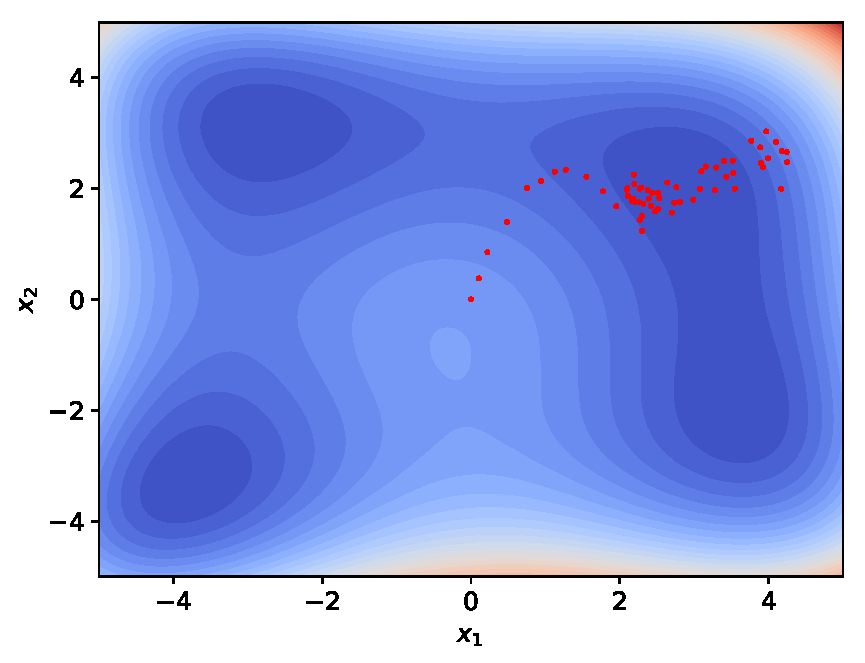
\includegraphics[height=5.8cm]{graphics/var-opt-conv/VO-R-himmelblau-convergence.pdf}
        \caption{}
        \label{fig: Theory: var-opt-conv-VO-R-himmelblau-convergence}
    \end{subfigure}
    \hfill
    \begin{subfigure}[b]{0.49\textwidth}
        \centering
        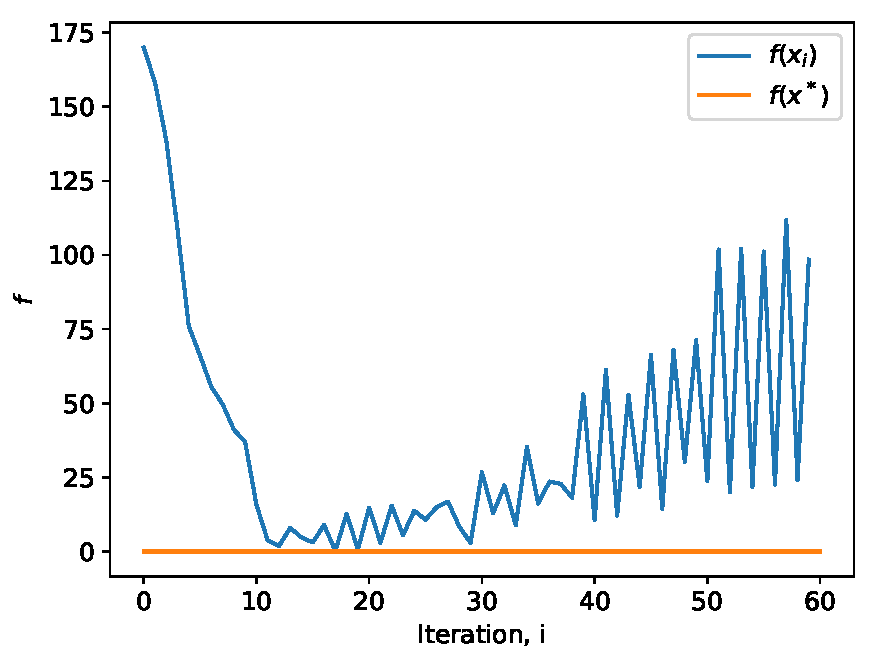
\includegraphics[height=5.8cm]{graphics/var-opt-conv/VO-R-himmelblau-f.pdf}
        \caption{}
        \label{fig: Theory: var-opt-conv-VO-R-himmelblau-f}
    \end{subfigure}
    \caption{\subref{fig: Theory: var-opt-conv-VO-R-himmelblau-convergence} Convergence of the \gls{VO} algorithm with isotropic Gaussian search distribution using regular gradients. \subref{fig: Theory: var-opt-conv-VO-R-himmelblau-f} Objective function value at each iteration. Similarly to the fixed variance version, a minimum is found, but the optimization of the variance drives it towards zero, resulting in larger gradients and instability.}
    \label{fig: Theory: var-opt-conv-VO-R-himmelblau}
\end{figure}
\begin{figure}[tbp!]
    \begin{subfigure}[b]{0.49\textwidth}
        \centering
        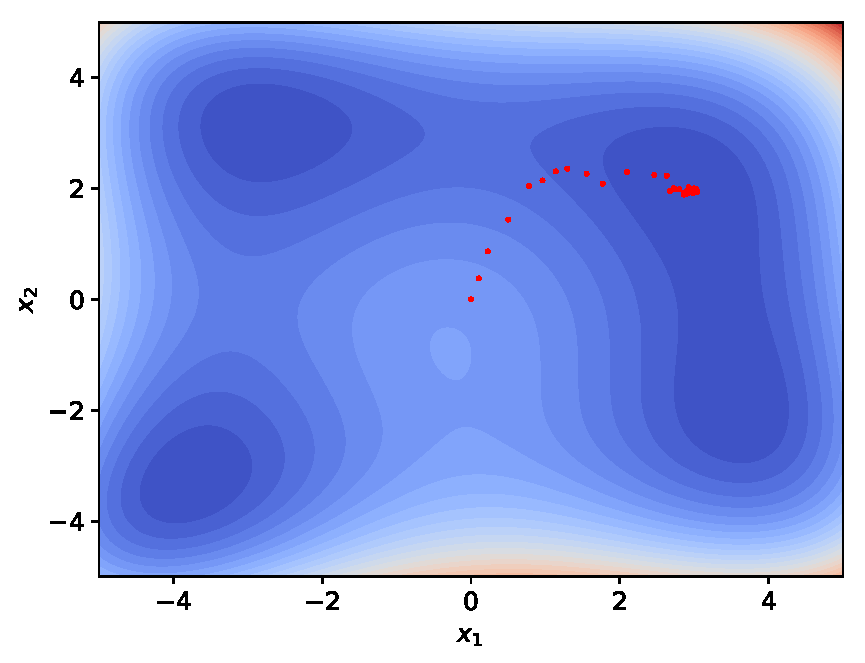
\includegraphics[height=5.8cm]{graphics/var-opt-conv/VO-N-himmelblau-convergence.pdf}
        \caption{}
        \label{fig: Theory: var-opt-conv-VO-N-himmelblau-convergence}
    \end{subfigure}
    \hfill
    \begin{subfigure}[b]{0.49\textwidth}
        \centering
        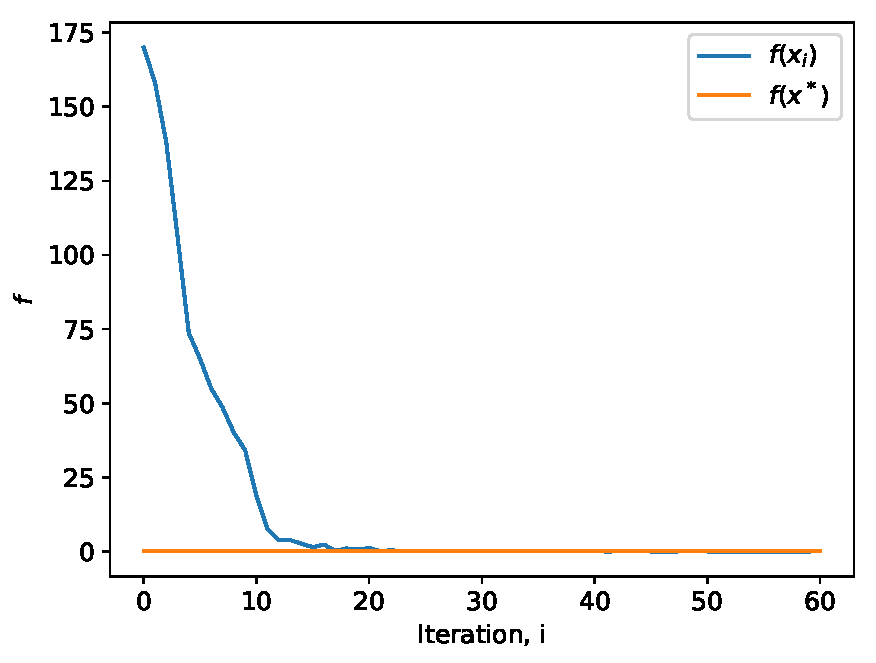
\includegraphics[height=5.8cm]{graphics/var-opt-conv/VO-N-himmelblau-f.pdf}
        \caption{}
        \label{fig: Theory: var-opt-conv-VO-N-himmelblau-f}
    \end{subfigure}
    \caption{\subref{fig: Theory: var-opt-conv-VO-N-himmelblau-convergence} Convergence of the \gls{VO} algorithm with isotropic Gaussian search distribution using natural gradients. \subref{fig: Theory: var-opt-conv-VO-N-himmelblau-f} Objective function value at each iteration. A minimum is found and the optimization of the variance drives the gradients toward zero resulting in convergence to the optimum.}
    \label{fig: Theory: var-opt-conv-VO-N-himmelblau}
\end{figure}